\chapter{Overview of the Cosmos SDK}
\label{OCS:overview}

In this chapter, we delve into the architecture of the Cosmos SDK, its modular components, and functionalities. We aim to shed light on both the advantages and the challenges faced by developers when employing this framework in blockchain development.

\section{High-level Overview}

The Cosmos SDK is an open-source framework designed to facilitate the creation of blockchain applications. Distinguished by its support for building application-specific blockchains, the Cosmos SDK departs from the traditional blockchain development model, which often relies on a single blockchain to support a wide range of applications. Instead, it provides the tools necessary for developers to construct bespoke blockchains tailored to the unique requirements of their specific applications. This capability is particularly evident in its role in creating both permissioned \gls{poa} and multi-asset public \gls{pos} blockchains, including notable implementations like the Cosmos Hub\cite{cosmos-hub}.

In contrast to traditional blockchains that utilize a universal virtual machine to execute a variety of smart contracts, the Cosmos SDK adopts a modular design. This architectural choice gives developers the flexibility to select and configure the components of their blockchain system. By enabling the customization of consensus mechanisms, governance models, and other blockchain parameters, the SDK allows for the optimization of each blockchain's efficiency, performance, and security. This emphasis on modularity and customization reflects a broader trend in blockchain development toward accommodating the diverse needs of different applications. The benefits of this approach, including improved performance and enhanced security measures, are illustrated in Listing~\ref{lst:app-based-blockchain}, which highlights the potential for achieving greater control and specificity in blockchain design using the Cosmos SDK\cite{kwon2019cosmos}.

The Cosmos SDK's approach also introduces significant advancements in blockchain interoperability and scalability. It aims to establish an interconnected ecosystem of blockchains, often referred to as the "Internet of Blockchains"~\cite{kwon2019cosmos}. This vision addresses a critical challenge in the blockchain community—the tendency for blockchains to operate in isolation, limiting their ability to interact and share information with one another. By promoting a structure that facilitates blockchain interconnectivity, the Cosmos SDK not only enhances the utility of individual blockchain projects but also contributes to a more cohesive and functional global blockchain landscape.

This introduction seeks to elucidate the core principles and capabilities of the Cosmos SDK. It underscores the framework's departure from traditional blockchain models towards a more flexible, application-specific approach. By doing so, the Cosmos SDK offers a powerful toolset for developers looking to leverage blockchain technology's benefits in a way that is closely aligned with their project's unique demands and objectives.

\begin{lstlisting}[language=bash, caption=Application based blockchains. Source:\cite{app-based-blockchain},label={lst:app-based-blockchain}]
                ^  +-------------------------------+  ^
                |  |                               |  |   Cosmos SDK
                |  |  State-machine = Application  |  |
                |  |                               |  v
                |  +-------------------------------+
                |  |                               |  ^
Blockchain node |  |           Consensus           |  |
                |  |                               |  |
                |  +-------------------------------+  |   CometBFT
                |  |                               |  |
                |  |           Networking          |  |
                |  |                               |  |
                v  +-------------------------------+  v
\end{lstlisting}

\section{Architecture}

Fundamentally, a blockchain functions as a replicated deterministic state machine as we saw in the previous chapter. When provided with an initial state \(S\) and a transaction \(T\), it generates a new state \(S'\), as illustrated in Listing \ref{lst:state-transition}.

\begin{lstlisting}[language=bash, caption=State machine transition. Source:\cite{app-based-blockchain},label={lst:state-transition}]
                +--------+                 +--------+
                |        |                 |        |
                |   S    +---------------->+   S'   |
                |        |    apply(T)     |        |
                +--------+                 +--------+
\end{lstlisting}

To enhance processing efficiency, transactions are grouped into blocks. The state machine transitions from state \(S\) to \(S'\) by processing a block of transactions \(B\), as detailed in Listing \ref{lst:state-block-transition}.

\begin{lstlisting}[language=bash, caption=Block of bundled transactions. Source:\cite{app-based-blockchain},label={lst:state-block-transition}]
            +--------+                              +--------+
            |        |                              |        |
            |   S    +----------------------------> |   S'   |
            |        |   For each T in B: apply(T)  |        |
            +--------+                              +--------+
\end{lstlisting}

The Cosmos SDK empowers developers with extensive flexibility in defining their application's state, transaction types, and the processes for state transition. We will further explore how to construct state machines using the Cosmos SDK in following sections.

\subsection{CometBFT}

CometBFT serves as the agnostic engine for both the networking and consensus layers of a blockchain (as seen in Listing~\ref{lst:app-based-blockchain}). It is responsible for organizing and propagating transaction bytes. Relying on the \gls{bft} algorithm developed by Tendermint, CometBFT achieves consensus among network nodes.

Validators, unique nodes within the network, are pivotal to the CometBFT consensus process. They are responsible for updating the blockchain with new transaction blocks. At any given time, a set of validators \(V\) is active, with one validator selected as the proposer for the next block. A block is considered valid if over two-thirds of \(V\) have signed a prevote and a precommit for it, and if all included transactions are verified as genuine. The validator set can be altered based on rules defined within the state machine. The simplicity of this process is encapsulated in Figure \ref{fig:cometbft-overview}.

\begin{figure}[H]
    \centering
    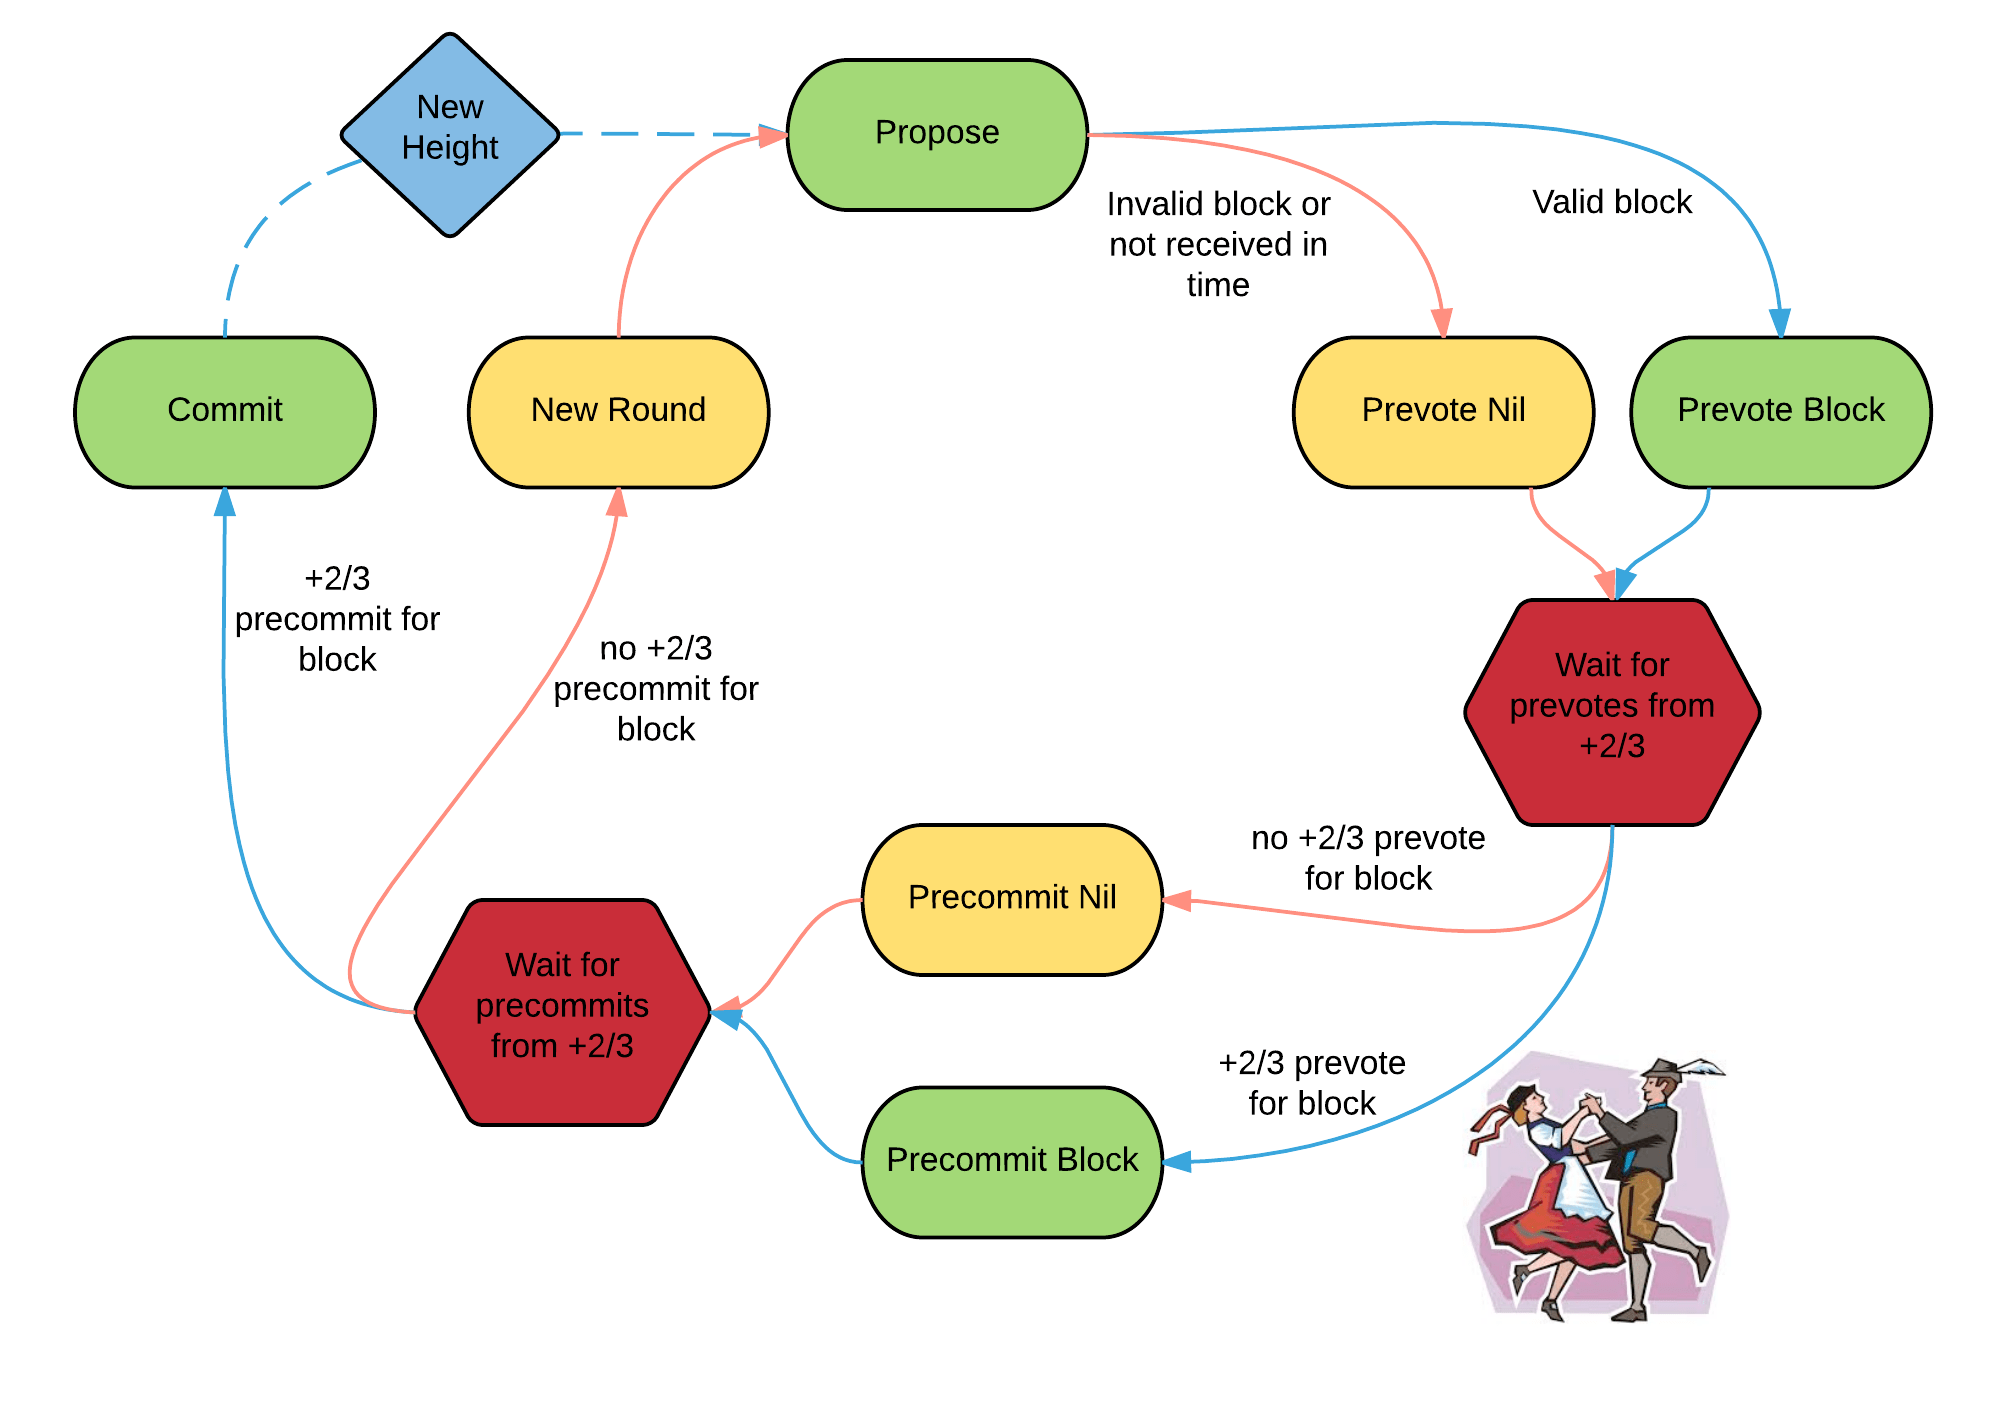
\includegraphics[width=\textwidth]{figures/cometbft.png}
    \caption{Consensus Overview CometBFT Source\cite{cometbft-overview}}
    \label{fig:cometbft-overview}
\end{figure}

\subsection{ABCI}

The \gls{abci} interface establishes standard protocols for communication between the consensus engine (CometBFT) and the application layer. This interface facilitates the separation of the consensus logic from application logic, significantly simplifying application development on the Cosmos SDK.

Through \gls{abci}, the consensus engine and the application interact seamlessly without needing to understand each other's internal mechanisms, as shown in Listing \ref{lst:ABCI}. This separation not only streamlines development but also promotes interoperability among various blockchain networks utilizing the Cosmos SDK.

\newpage
\begin{lstlisting}[language=bash, caption=ABCI Interface. Source:\cite{app-based-blockchain},label={lst:ABCI}]
                      +---------------------+
                      |                     |
                      |     Application     |
                      |                     |
                      +--------+---+--------+
                               ^   |
                               |   | ABCI
                               |   v
                      +--------+---+--------+
                      |                     |
                      |                     |
                      |       CometBFT      |
                      |                     |
                      |                     |
                      +---------------------+
\end{lstlisting}

\section{Applications Architecture}
\label{ch:applicatoins-architecture}

The Cosmos SDK provides a robust framework for blockchain application development, focusing on a modular and decoupled architecture. This design principle is crucial, allowing developers to concentrate on the application logic while the Cosmos SDK handles underlying functionalities. The \texttt{baseApp} acts as a fundamental template, routing transactions to various modules and facilitating communication with the CometBFT engine through \gls{abci} methods.

Modules within the Cosmos SDK serve as mini state machines within the overarching blockchain ecosystem, defining segments of the state and specific message types. The \texttt{baseApp} efficiently routes these messages to the appropriate modules, which then use Protobuf definitions to interpret these messages, turning byte transactions managed by CometBFT into actionable logic for applications.

As illustrated in Figure \ref{fig:application-modules}, the Cosmos SDK's architecture showcases the application layer's general structure. The SDK's core manages essential connections and module composition, setting the stage for developers to implement custom modules. These modules, developed using the SDK, enact the application's primary functionalities, demonstrating the SDK's capacity to support sophisticated blockchain application development.

\begin{figure}[H]
    \centering
    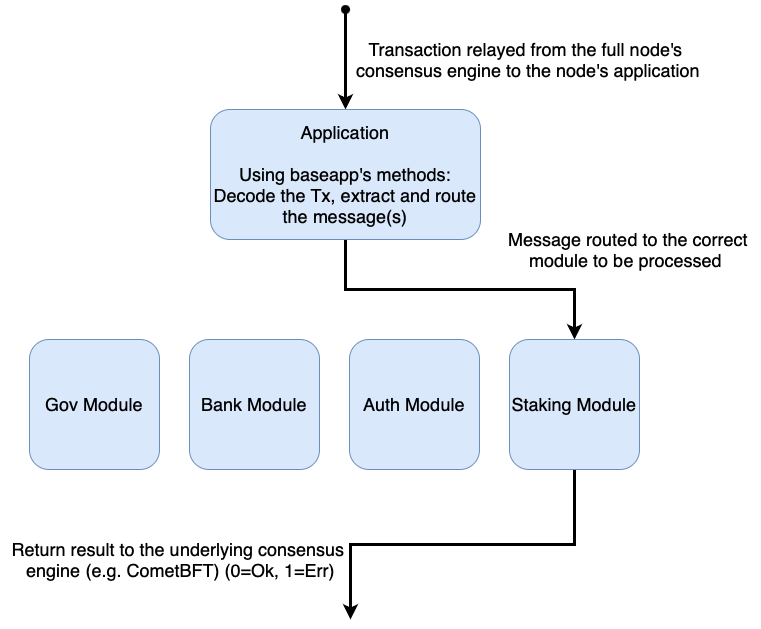
\includegraphics[width=\textwidth]{figures/prueba.png}
    \caption{Application architecture}
    \label{fig:application-modules}
\end{figure}

This architectural approach offers several benefits. It promotes functionality encapsulation, making applications easier to develop, maintain, and scale. Moreover, it enhances applications' interoperability and scalability built with the Cosmos SDK, as modules can be interchanged, updated, or extended without impacting the system's overall integrity. Additionally, this modular design encourages a collaborative development environment, where shared modules and best practices accelerate the blockchain application development process.


\section{Cosmos SDK Approach to Smart Contracts}
\label{sec:cosmos-sdk-smart-contracts}

The Cosmos SDK offers a distinctive framework for smart contracts, which contrasts with the \gls{evm} based model in several key aspects. This approach fundamentally alters the development experience, addressing some of the challenges inherent in the \gls{evm} model while providing developers with greater flexibility and efficiency.

\subsection{Comparison with EVM-based Smart Contracts}
\label{subsec:comparison-with-evm}

\gls{evm} based smart contracts are executed within a global, deterministic virtual machine, ensuring that contracts run identically on every node of the network. This model offers predictability and a high degree of security through immutability; once deployed, the code of a smart contract cannot be altered. However, this immutability also presents significant challenges. For instance, any bugs or vulnerabilities in the code are permanent and can lead to security risks or loss of funds with no direct path for correction.

In contrast, the Cosmos SDK does not rely on a universal virtual machine for contract execution. Instead, it enables the creation of application-specific blockchains, where smart contracts are integrated as part of the blockchain protocol itself. This architecture allows for contracts to be upgraded or modified as part of the chain's governance process, providing a more flexible approach to managing and improving contract logic over time.

\subsection{Improvements in Development Experience}
\label{subsec:improvements-in-development}

The Cosmos SDK framework significantly improves the smart contract development experience through its modular architecture and flexibility. Developers can build highly customized blockchains tailored to their application's specific needs. This modularity extends to smart contracts, where the logic can be encapsulated within modules that are easily upgradeable and interoperable with other blockchains in the Cosmos ecosystem.

One of the primary advantages of this approach is the ability to fix bugs or update smart contract logic without the need for complex and risky migration strategies. Since contracts are part of the blockchain protocol, updates can be proposed, voted on, and implemented through the chain's governance mechanism. This approach not only enhances security but also enables continuous improvement and adaptation of contract functionality to meet evolving requirements.

Furthermore, the Cosmos SDK's focus on interoperability through the \gls{ibc} protocol opens up new possibilities for smart contracts to interact across different blockchains. This capability enables a more connected and efficient blockchain ecosystem, where contracts can leverage resources, assets, and functionalities from various chains.

